\chapter{Vizualizace skrze programovatelný logický automat}
V této kapitole se nachází popis jednotlivých částí ovládání instalace skrze PLC firmy TECO - CP-2007 \cite{TECO}, které obashuje knihovny pro práci s KNX/IP \cite{KNXlib} a MQTT \cite{MQTTlib} a dále integrovaný webový server pro vizualizaci \cite{WebMaker}. Všechny tyto části jsou podrobněji rozvedeny v následujících podkapitolách.
Ovládání a vizualizace instalace je možné provádět i skrze PLC jiných výrobců za předpokladu, že mají implementované knihovny pro komunikace KNX/IP a MQTT. PLC výrobce TECO bylo vybráno kvůli jeho specializaci na domácí automatizaci, dostupnosti a ceně.
\section{CP - 2007}
Jedná se základní modul řídícího systému Foxtrot, který je vyroben pro přichycení na DIN Lištu. Obsahuje 2 ethernet porty, 2 sériové porty, 15 vstupů z nichž je 14 univerzálních a 1 galvanicky oddělený digitální, 15 výstupů z nichž je 11 releových a 4 analogové. Dále pak obsahuje 2 sloty na rozšiřující moduly. \cite{TECO}

\begin{figure}[!ht]
    \begin{center}
        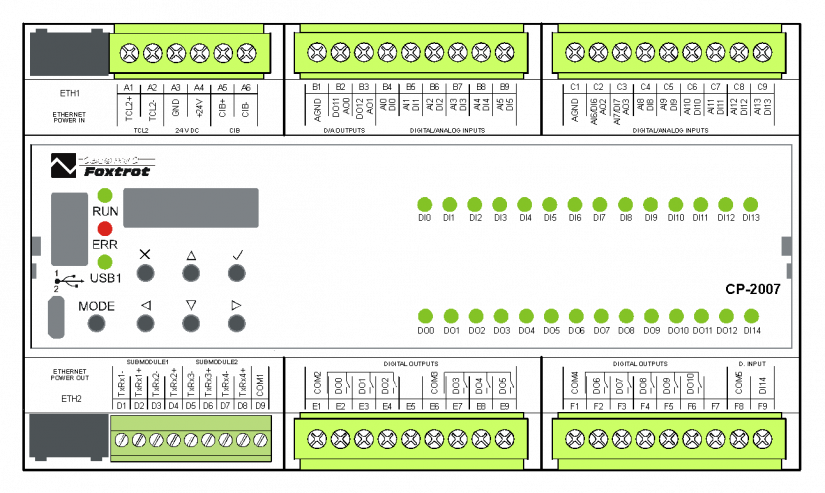
\includegraphics[scale=0.7]{obrazky/CP-2007.png}
    \end{center}
    \caption[CP-2007 \cite{TECO}]{CP-2007 \cite{TECO}}
    \label{fig:CP-2007}
\end{figure}

\section{Ovládací prvky}
\section{Komunikace KNX/IP}
\section{Komunikace MQTT}
\section{Web Server}